\documentclass{beamer}
\usepackage{hyperref}
\renewcommand{\matrix}[2]{ \left(\begin{array}{#1} #2 \end{array}\right)}
%../../../papers/PJTpreamble.tex
\begin{document}

\title{INFINITESIMAL PHASE RESPONSE CURVES FOR PIECEWISE LINEAR DYNAMICAL SYSTEMS}
%\subtitle{Subtitle}
\author % (optional, for multiple authors)
{Youngmin Park\inst{1}\\
Advisors: Peter J. Thomas\inst{1}, Hillel J. Chiel\inst{2}
With help from Kendrick M. Shaw\inst{3}}
\institute % (optional)
{
  \inst{1}%
  Department of Mathematics
  \inst{2}%
  Department of Biology
  \inst{3}%
  MSTP Program at CWRU Medical School
  
  Case Western Reserve University
}
\frame{\titlepage}


% 
% \begin{frame}\frametitle{PJT comments}
% \begin{enumerate}
% \tiny
%\item Motivation: 1. Biological Oscillators. 2. (why) Phase Response Curves (matter) (and note the iPRC cannot be solved for analytically except in a few cases, which you should be familiar with; use Morris Lecar as an example of one you cannot find analytically). 3. Piecewise linear flows arise in several contexts: Glass networks, Coombes/McKean model,  Shaw et al's ``iris model", which is a piecewise linear analog of the ``sine'' SHC system, which in turn is motivated by influence of passage near a fixed point on response of limit cycle to perturbations.  

% 2: the motivation for PRC from a general biological level is OK -- many process in nature are cyclic, including motions produced by animals.  An active area of research in mathematical bio is in trying to understand how animals control their own movements.  At a general level, how do you incorporate information from the world to how you're moving. Mathematically the form that rhythmic systems take tend to involve a limit cycle (period orbit that nearby solutions converge to it; isolated (non-Hamiltonian), periodic orbit). typically use stable limit cycles in modeling CPGs (interested in modeling CPGS can be modeled using stable LC).

% john gukenheimer 1980 isochrons and phaseless sets (...math. biol.) -- information on isochrons

%once w ehave a LC, how do we quantify effects of perturbations -- can label points in BA by where they arrive at the LC (isochrons).  In iPRCs we assume perturbations are weak. We end up speeding it up or slowing it down => directional derivate

%The ongoing context for this work involves how sensitive the system is to perturbations (patterned inputs from body)

% typically ODE's are smooth, but don't have to be for LC's.

% focus on the PRC as quickly as possible -- develop as clearly and succinctly as possible.

%\item Put results on PWL flows and the adjoint before discussing the kink in the iris system and iPRC in arc length?  You can mention that the peak sensitivity lies in at the boundary and in a similar locus for the sine SHC, but we don't really have a complete answer as to why that is.  The PWL adjoint solution is much more complete at this point.
%\item You can talk about the kink and also the iPRC via arc length for Morris-Lecar at the end, under ``future work".
%\item ``biological motivation slide": motivation is to understand how response of a limit cycle trajectory to external perturbations changes when the LC passes near a fixed point.  The origin of this question is in thinking about how one incorporates proprioceptive feedback to modulate the tempo of a CPG.  But for the MS thesis the focus should be more on the mathematical questions that result.  You can certainly mention \textit{Aplysia} (since Prof. Chiel will be there!) but not make it a focus, I think.
%\item To define phase, 1. introduce a deterministic ODE system with smooth right hand side; 2. introduce a limit cycle and its basin of attraction; 3. introduce the isochron or phase function in this context.  You can't just jump in with "the phase of a limit cycle is a number..."  The phase function is a map from the underlying point space (the basin of attraction of the LC, which is some open subset of $\mathbb{R}^2$ for the ML system) to the circle $\mathcal{S}^1$, parametrized as $\theta(x)\in[0,1)$.
%\item the iPRC is \emph{defined} as a derivative -- it is the directional derivative of $\theta(x)$ in the direction of the perturbation.  (not quite ``The iPRC is equivalent to the gradient of the isochron function over a limit cycle.'') Then you should give the argument for why it satisfies the adjoint equation.
%\item You can introduce the models earlier in the introduction section, provided you explain why each is relevant to the discussion.  And break them up, and show a picture for each.  The pictures can come from Shaw et al provided you cite.
%\item slide 11: does the iris iPRC resemble ML or does it resemble the sine system?
%\item iPRC and arc length: we have numerical results but no theory.  skip this part until there is a theory.  We can discuss your two Lemmas, but I don't think the story is there yet?  You can come back to it, but put the strongest part of the story first, to allay any concerns in the committee over the substance of the thesis.
%\item The start of the PWL section looks good so far.  It would help a lot to have one big diagram with everything labeled, something like what's in my notes.  
% \end{enumerate}
% \normalsize
% \end{frame}

\begin{frame}
\frametitle{Table of Contents}
\tableofcontents%[currentsection]
\end{frame}

\section{Introduction}
\subsection{Motivation}

\begin{frame}
  \frametitle{\insertsection}
  \framesubtitle{\insertsubsection}

  \begin{itemize}
  \item Biological oscillators
  \item Phase response curves
  \item Piecewise linear flows
  \begin{itemize}
  \item Gene regulatory (Glass) networks
  \item Piecewise linear neuronal models (Coombes 2008)
  \item ``Iris system'' (Shaw et al 2012 \cite{ShawParkChielThomas2012SIADS})%, a piecewise linear analog of the sine SHC system.
  \end{itemize}
  \end{itemize}

  %\item Interested in the underlying structure of the feeding mechanism in \textit{Aplysia Californica}
  %	\begin{itemize}
  %	\item A special case of a central pattern generator (CPG)
  %	\end{itemize}
  %\item The results of Shaw et al. (2012) are the results of theoretical perturbative analysis on candidate models for the feeding mechanism.
\end{frame}
  
\subsection{The phase response curve}

\begin{frame}
\frametitle{\insertsection}
  \framesubtitle{\insertsubsection}
  Consider a deterministic system of ODEs in $\mathbb{R}^n$:
  \begin{equation}
  \frac{dx}{dt} = F(x),
  \end{equation}

  where $F$ is a smooth map $F:\mathbb{R}^n \rightarrow \mathbb{R}^n$. Let the system have a solution $\gamma$, which represents a (non-Hamiltonian) isolated periodic orbit with period $T$,
  \begin{equation}
  \gamma(t) = \gamma(t+T),
  \end{equation}

  such that nearby solutions converge to it as $t \rightarrow \infty$.  We call this a stable limit cycle.  Note: the set of initial conditions that converge to the limit cycle is called the basin of attraction ($BA$).

  
  

\end{frame}


\begin{frame}

  \begin{definition} The \underline{phase} of a limit cycle with period $T$ is a function $\theta: \gamma \rightarrow S^1$ with $S^1$ parameterized as $\theta(\gamma(t)) \in [0,1)$ and
  \begin{equation}
  \frac{d }{dt}\left (\theta(\gamma(t)) \right ) = 1/T \mod 1,
  \end{equation}
  \end{definition}
  where $\theta = 0$ is chosen arbitrarily.


\end{frame}

\begin{frame}
   \begin{figure}
   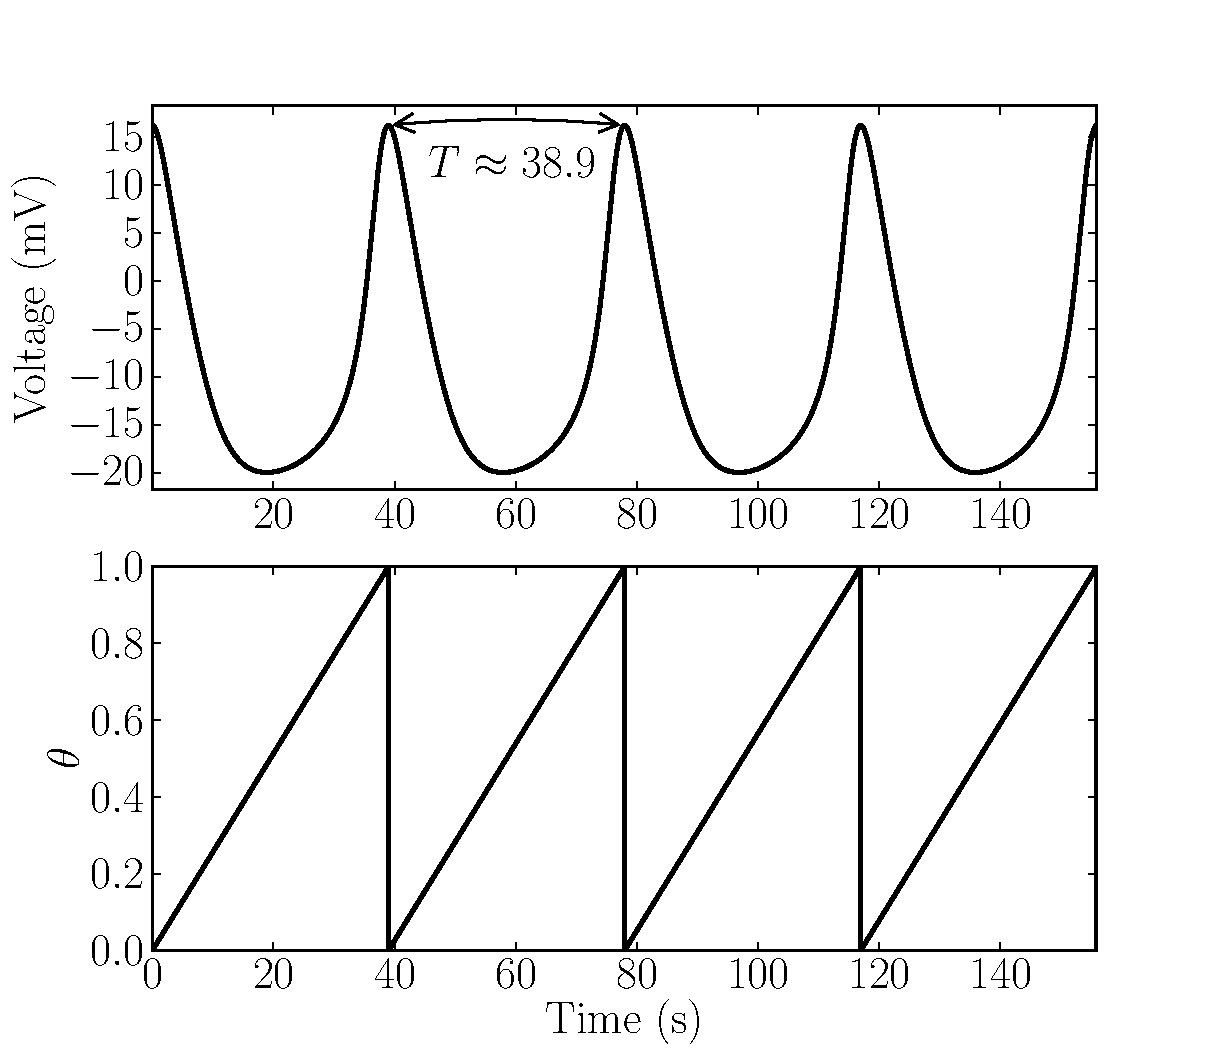
\includegraphics[width=\textwidth]{dthetadt_fig.pdf}
  \end{figure}

\end{frame}


  \begin{frame}
    \begin{definition}
  Given a point $x_0 \in BA$, there exists a unique $\theta(x_0)$ such that 
  \begin{equation}
    \lim_{t \rightarrow \infty} | x(t) - \gamma(t + T\theta(x_0))  | \rightarrow 0,
  \end{equation}
  
  The value $\theta(x_0)$ is the \underline{asymptotic phase} of the point $x_0$.

  \end{definition}

  \begin{definition}
  An \underline{isochron} is a level curve consisting of points that share the same asymptotic phase.
  
%   For a trajectory $x(t)$ with initial condition $x_0 \in BA$, there exists a unique $\theta(x_0)$ such that
%   \begin{equation}
%     \lim_{t \rightarrow \infty} | x(t) - \gamma(t + T\theta(x_0))  | \rightarrow 0,
%   \end{equation}
%   
%   then these points are on the same isochron. 
  \end{definition}
   Note: all points on the isochron share the same asymptotic phase, so $\forall x \in BA$,
  \begin{equation}
   \frac{d\theta(x)}{dt} = 1/T.
  \end{equation}
  
  \end{frame}
  
  \begin{frame}
  \begin{figure}
   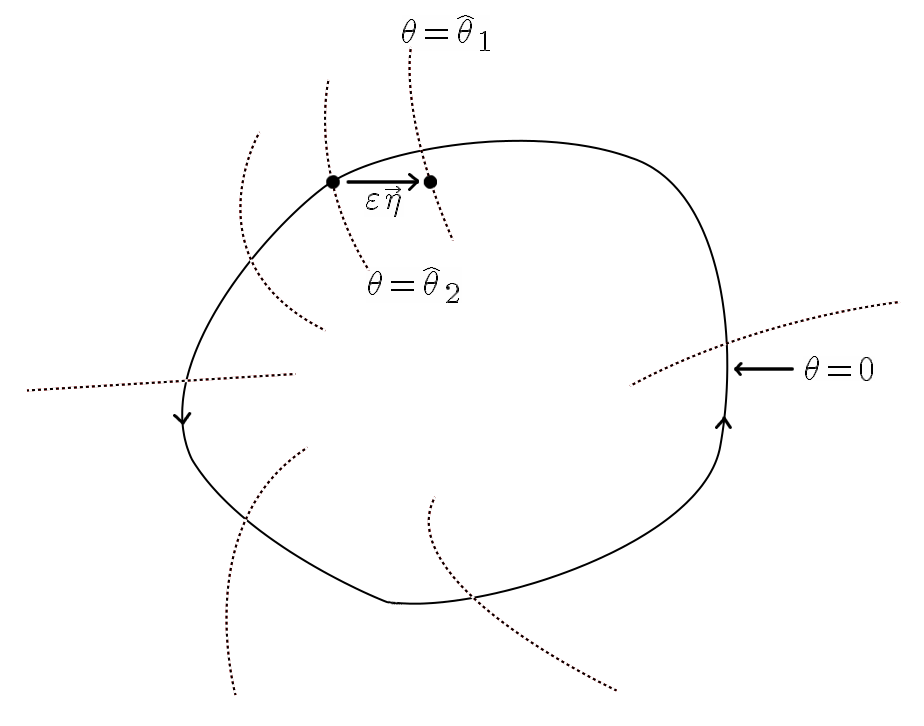
\includegraphics[width=\textwidth]{isochron-demo.png}
  \end{figure}

   
  \end{frame}

  
\begin{frame}
Suppose we perturb a limit cycle with a perturbation of size $\varepsilon$ in the unit vector direction $\eta$.  How does the asymptotic phase of the perturbed trajectory compare to the phase of the unperturbed trajectory?

\begin{equation}
\theta(\gamma(t) + \varepsilon \eta) = \theta(\gamma(t)) + \varepsilon D\theta(\gamma(t))\cdot \eta + O(\varepsilon^2).
\end{equation}

\begin{equation}
\Delta \theta = \theta(\gamma(t) + \varepsilon \eta) - \theta(\gamma(t)) = \varepsilon D\theta(\gamma(t))\cdot \eta + O(\varepsilon^2).
\end{equation}

\begin{equation}
\lim_{\varepsilon \rightarrow 0} \frac{\Delta \theta}{\varepsilon} = D\theta(\gamma(t))\cdot \eta =: z(t) \cdot \eta
\end{equation}

\begin{itemize}
 \item An explicit expression for $z(t)$ exists for a small number of cases.
\end{itemize}
\end{frame}


% \begin{frame}
% One way to solve for the iPRC is by using the adjoint equation.  The linearization about the limit cycle $\gamma$ satisfies the equation
% \begin{equation}
%  \frac{dy}{dt} = DF(\gamma(t)) y(t),
% \end{equation}
% 
% where $y(t)$ is an arbitrary, small perturbation.
% \begin{equation}
% \begin{split}
%  0 &= \frac{d}{dt} (z(t)\cdot y(t))\\
%  &=\frac{dz}{dt}\cdot y(t) +z(t)\cdot\frac{dy}{dt}\\
%  &=\frac{dz}{dt}\cdot y(t) +z(t)\cdot DF(\gamma(t)) y(t)\\
%  &=\frac{dz}{dt}\cdot y(t) +DF(\gamma(t))^T z(t) \cdot y(t)\\
%  &=\left [ \frac{dz}{dt} +DF(\gamma(t))^T z(t)\right ] y(t).
%  \end{split}
% \end{equation}
% \end{frame}

  \begin{frame}
 \frametitle{\insertsection}
    	\framesubtitle{\insertsubsection}
    \begin{figure}
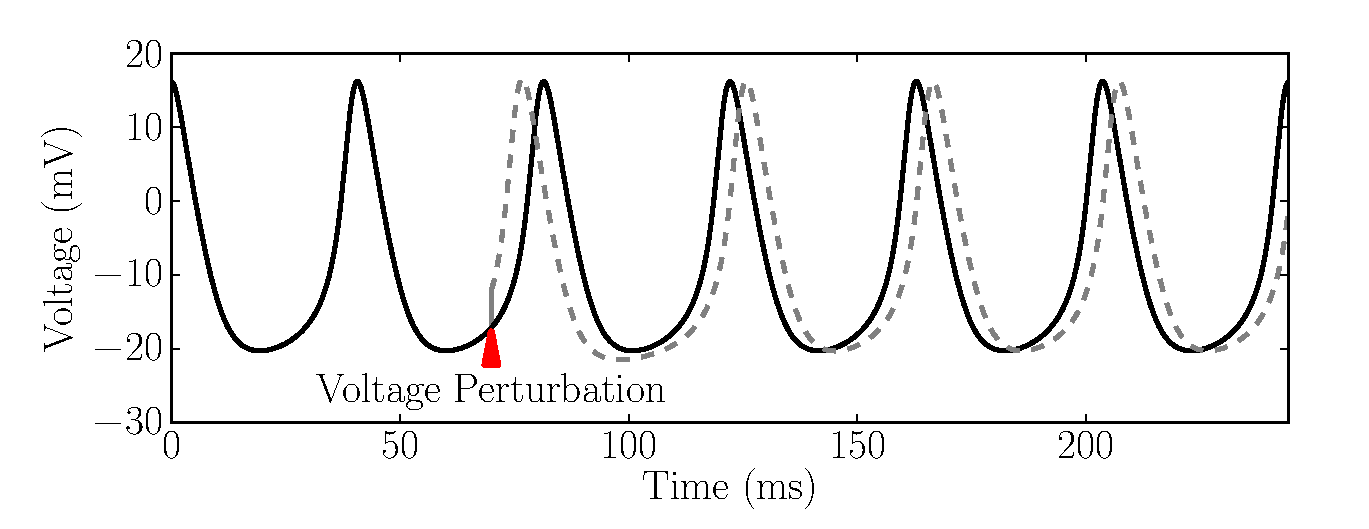
\includegraphics[width=1\textwidth]{voltage-pert-ml-vt.png}
\caption{Example of a phase response for the Morris-Lecar model: a voltage perturbation at phase $\phi \approx .6$ ($t \approx 70ms$) of a limit cycle leads to a change in timing of $\Delta \theta \approx .1$.  }
\end{figure}
  \end{frame}

  \begin{frame}
 \frametitle{\insertsection}
    	\framesubtitle{\insertsubsection}
    \begin{figure}
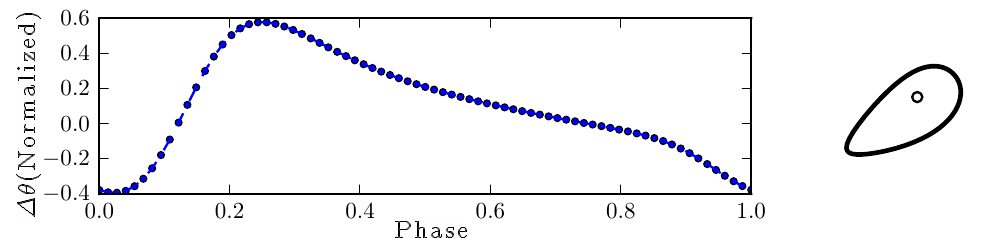
\includegraphics[width=1\textwidth]{voltage-pert-ml-quarter.png}
\caption{Example of an iPRC: Blue dots indicate the phase at which we apply an infinitesimal perturbation of size 1e-4 to the same model. The resulting phase difference is shown along the vertical axis.  The voltage over time plot from before is now shown in a phase space representation on the right.}
\end{figure}
  \end{frame}



\begin{frame}
 The iPRC, $z(t)$, satisfies the adjoint equation
\begin{equation}
 \frac{dz}{dt} = -DF(\gamma(t))^T z(t).
\end{equation}

Notes:
\begin{itemize}
 \item Provides another way to calculate the iPRC
 \item 
\end{itemize}


\end{frame}


\subsection{Assumptions for piecewise linear dynamical systems}
\begin{frame}
\frametitle{\insertsection}
  \framesubtitle{\insertsubsection}

   By piecewise linear differential equations, we mean the following: Let $B \subset \mathbb{R}^n$.  A vector field $F:B \rightarrow \mathbb{R}^n$ is piecewise smooth on $B$ if there exists a finite number of open sets such that
   \begin{itemize}
    \item $B_i \cap B_j = \varnothing, \forall i \neq j$
    \item $B = \bigcup_{k=1}^n \overline{B}_k$
    \item $F^k(x) = \chi_k(x) F(x)$ is smooth
   \end{itemize}
  where $\chi_k(x)$ is the characteristic function of $B_k$ and $||F|| < \infty$.
   
   For the systems we consider, adjacent vector fields, $F^k, F^{k+1}$ ``flow'' in the same direction at each boundary, and each vector field is defined by a system of linear equations.  We further assume that such systems have limit cycles.
\end{frame}


\begin{frame}
\begin{figure}
\frametitle{\insertsection}
  \framesubtitle{\insertsubsection}
 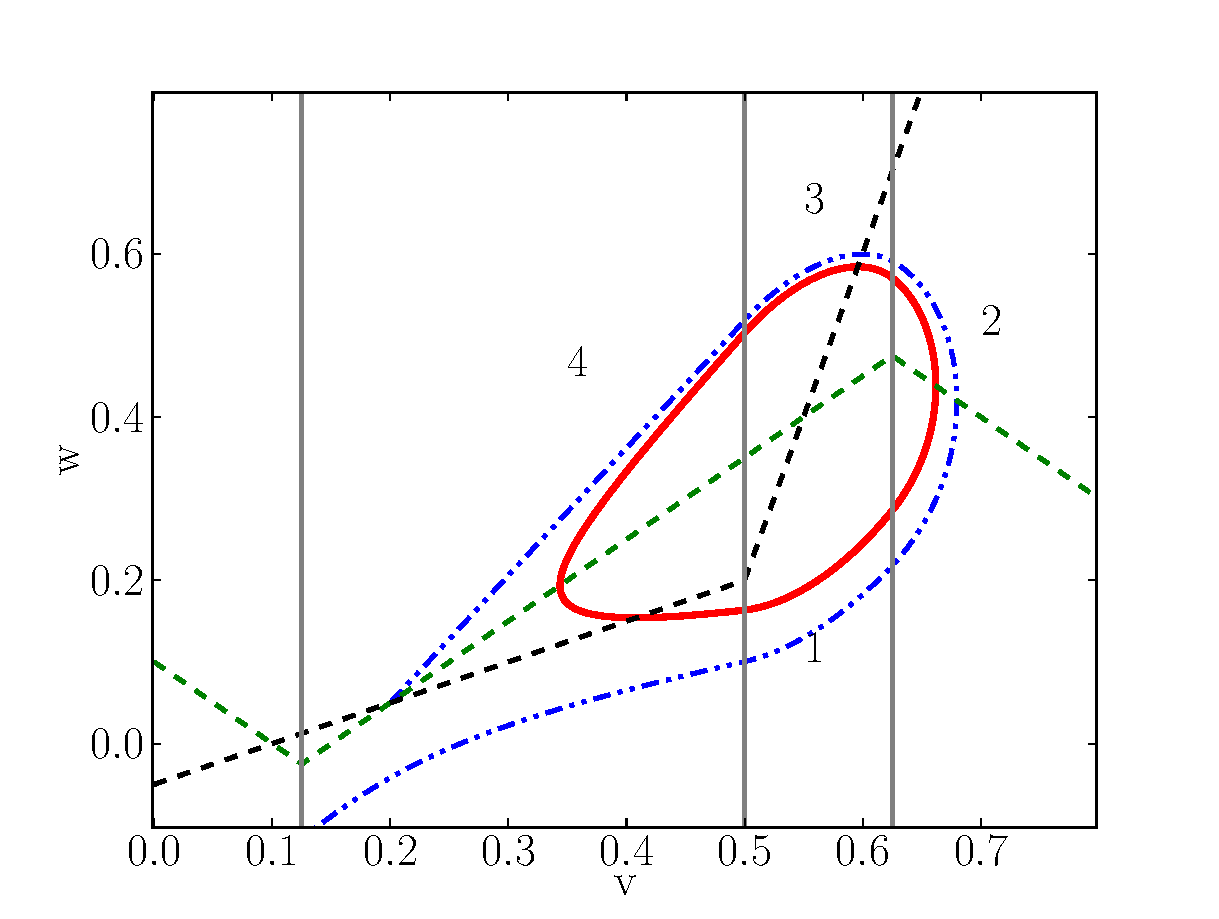
\includegraphics[width=.8\textwidth]{pml_fig.pdf}
 \caption{Example of a piecewise linear differential equation: Piecewise Morris-Lecar model (Coombes 2008 \cite{Coombes:2008:SIADS}).}
\end{figure}
\end{frame}

\begin{frame}
 \begin{figure}
 \frametitle{\insertsection}
  \framesubtitle{\insertsubsection}
  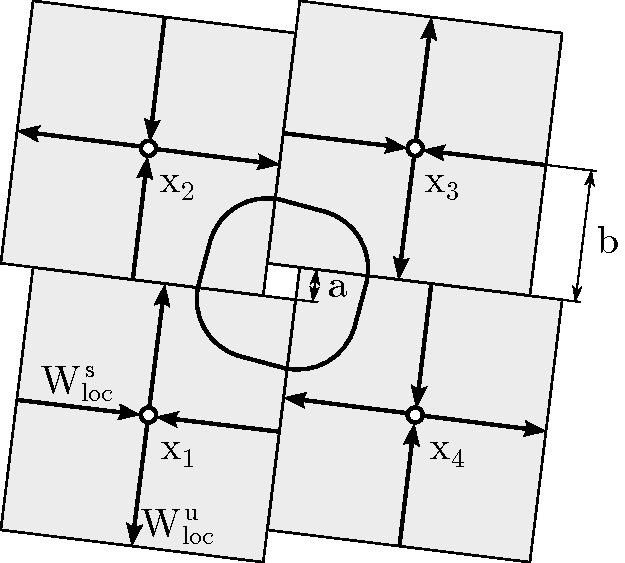
\includegraphics[width=.5\textwidth]{sine_to_iris_fig_sketch_iris.pdf}
  \caption{Example of a piecewise linear differential equation: Iris system (Shaw et al 2012).}
 \end{figure}
\end{frame}


\begin{frame}
  For piecewise smooth dynamical systems, we assume the following without proof:
  \begin{itemize}
   \item Trajectories exist and are unique for all time
   \item The limit cycle is stable and has an open basin of attraction
   \item The limit cycle has well-defined phase with $\frac{d\theta}{dt} = 1/T$
   \item A unique asymptotic phase exists for each point in the basin of attraction
   \item Isochrons exist and are continuous
   \item $\frac{d\theta(x)}{dt} = 1/T$ for all points in the basin of attraction
  \end{itemize}
\end{frame}

\begin{frame}
 \begin{figure}
 \frametitle{\insertsection}
  \framesubtitle{\insertsubsection}
  \includegraphics[width=.6\textwidth]{iris_isochron_fig-revised.pdf}
  \caption{Isochrons in the iris system (Shaw et al 2012).}
 \end{figure}
\end{frame}


\begin{frame}
Recall the derivation of the iPRC,
\begin{equation}
\lim_{\varepsilon \rightarrow 0} \frac{\Delta \theta}{\varepsilon} = D\theta(\gamma(t))\cdot \eta =: z(t) \cdot \eta.
\end{equation}
This description of the iPRC may not accurately describe the effects of perturbations up to a finite number of phases (boundary crossings).

We now show how to calculate the iPRC for points where this formula is invalid.
  \end{frame}


  
  
% \begin{frame}
%   \frametitle{\insertsection}
%   \framesubtitle{\insertsubsection}
%   \begin{definition} The \underline{phase response} of a limit cycle is the change in phase given a perturbation at some phase along the limit cycle.  The \underline{phase response curve} (PRC) is the collection of phase changes plotted over respective phase values.  The \underline{infinitesimal phase response curve} (iPRC) is constructed using infinitesimally small perturbations.
%   \end{definition}
% \end{frame}
% 
%   



\section{Solving the adjoint equation over boundaries of PWL systems}
\begin{frame}
\frametitle{Table of Contents}
\tableofcontents[currentsection]
\end{frame}



\subsection{General equation for discontinuous jumps across boundaries of planar systems}
  \begin{frame}
 \frametitle{\insertsection}
    	\framesubtitle{\insertsubsection}
We first fix notation and define terms before introducing the theorem.   Let $F^R$ denote the vector field of region $R$, where each region is numbered according to the direction of flow.  Given a limit cycle $\gamma$ with period $T$, we denote the final and initial values of a vector field along the limit cycle as
\begin{equation}
\begin{split}
F^R_f &= F^R(\gamma^R(t_R)),\\
F^{R+1}_0 &= F^{R+1}(\gamma^{R+1}(0)),
\end{split}
\end{equation}
where time is ``local'' and $t_R$ denotes the time of flight through region R.  Let
\begin{equation}
 F^{R} = (f^{R}, g^{R}).
\end{equation}



  \end{frame}
  
% \begin{frame}
% \frametitle{\insertsection}
% \framesubtitle{\insertsubsection}
% An equivalent solution to the perturbative derivation of the iPRC uses the adjoint equation.  The solution to the adjoint equation,
% 
% \begin{equation}
%  \frac{dz}{dt} = -\left[ DF^R(\gamma(t)) \right ]^T z(t),
% \end{equation}
% 
% for over the limit cycle $\gamma$ is the iPRC.  The iPRC may also be defined by the gradient of the phase function,
% 
% \begin{equation}
%  z(t) \equiv \nabla \theta(\gamma(t)).
% \end{equation}
% 
% \end{frame}
  
  \begin{frame}
  \frametitle{\insertsection}
   \framesubtitle{\insertsubsection}
   Recall
   \begin{equation}
    \frac{dz^R}{dt} = A^R z(t)^R.
   \end{equation}

    Let
    \begin{itemize}
     \item $\hat{n} = (\cos\psi_R, \sin\psi_R)$ denote the vector normal to a linear boundary and $\hat{w} = (-\sin\psi_R, \cos\psi_R)$ denote the vector tangent to the boundary.
     \item $z_f^R=\lim_{t\to t_R^-}z(t)$ be the value of the adjoint equation at the end of region R.
     \item $z_0^{R+1}=\lim_{t\to 0^+}z(t)$ be the new value after the jump induced by the boundary. 
    \end{itemize}
  \end{frame}

  \begin{frame}
   \frametitle{\insertsection}
   \framesubtitle{\insertsubsection}
\begin{theorem}
 We can calculate discontinuities of the iPRC over boundaries of a piecewise linear planar system by the following relation
 \begin{equation}
z_0^{R+1}=M^R z_f^R,
\end{equation}

where
\begin{equation}
M^R = \matrix{cc}{f_0^{R+1} & g_0^{R+1}\\
-\sin\psi_R & \cos\psi_R}^{-1}\matrix{cc}{f_f^R & g_f^R\\
-\sin\psi_R & \cos\psi_R},
\end{equation}
where $F_0^{R+1}\cdot \hat{n} > 0$
\end{theorem}
\end{frame}


\begin{frame}
\frametitle{\insertsection}
\framesubtitle{\insertsubsection}
\textit{Proof}. 
Consider a linear boundary between two piecewise linear systems, each defined by
\begin{eqnarray}
\frac{dx}{dt}&=&F^R(x)\\
\frac{dx}{dt}&=&F^{R+1}(x),
\end{eqnarray}
Where $F^R$ and $F^{R+1}$ are smooth functions within their respective domains.  Trajectory solutions in each region satisfies each system, with continuity enforced across the boundary. (If $x(t)$ is a solution in the $BA$, then $x^{R+1}(0) = x^R(t_R)$).
\end{frame}


\subsection{Proof}
\begin{frame}
\frametitle{\insertsection}
\framesubtitle{\insertsubsection}
By the use of the chain rule, we have the useful relation,
\begin{equation}
 \frac{d\theta}{dt}=F^{R/R+1}(x(t))\cdot\nabla\theta(x(t)).
\end{equation}

In addition, the change in phase $d\theta/dt$ must satisfy a constant differential equation over all regions and boundaries, which gives us a relation between $z_0^{R+1}$ and $z_f^{R}$:

\begin{equation}\label{eq:thetaflow}
F_0^{R+1}\cdot z_0^{R+1}=F_f^{R}\cdot z_f^{R}=\frac{1}{T}.
\end{equation}
\end{frame}


% \begin{frame}
% \frametitle{\insertsection}
% \framesubtitle{\insertsubsection}
% Next, consider the isochron over the boundary.
%     \begin{definition} An \underline{isochron} is the set of points that have the same asymptotic phase.  Suppose $\gamma(t)$ is a stable limit cycle with period T.  Then for each point $x$ in the basin of attraction of $\gamma$ there exists a unique phase $\theta(x)$ such that 
% \begin{equation}
% \lim_{t \rightarrow \infty} | x(t) - \gamma(t + T\theta(x))| = 0,
% \end{equation}
% where $x(t)$ is a trajectory of a dynamical system with $x(0) = x$.
% \end{definition}
% The iPRC is equivalent to the gradient of the isochron function over a limit cycle.
% \end{frame}


\begin{frame}
\frametitle{\insertsection}
\framesubtitle{\insertsubsection}
Let $\theta(x)$ be the asymptotic phase function as defined before.  The function $\theta(x)$ must be continuous along the boundary with respect to space (though not necessarily differentiable).

Let the interval $(w_{min},w_{max})$ lie in the basin of attraction, with $w_0=0$ the crossing point of the limit cycle.  Then for each isochron,
\begin{equation}
\theta^{R+1}(w) = \theta^R(w).
\end{equation}
\end{frame}

\begin{frame}
\frametitle{\insertsection}
\framesubtitle{\insertsubsection}
For the systems we consider, $\theta(w)$ is differentiable in the direction of the coordinate $w$, so
\begin{equation}
\left(\nabla\theta^{R+1}(w)\right)\cdot\hat{w}=\left(\nabla\theta^R(w)\right)\cdot\hat{w}.
\end{equation}

In particular, for $w = 0$,
\begin{equation}
 z_0^{R+1}\cdot\hat{w}=z_f^{R}\cdot\hat{w}.
\end{equation}
\end{frame}


\begin{frame}
\frametitle{\insertsection}
\framesubtitle{\insertsubsection}
Given the equations 
\begin{equation}
\begin{split}
 F_0^{R+1}\cdot z_0^{R+1}&=F_f^{R}\cdot z_f^{R},\\
 \hat{w}\cdot z_0^{R+1}&=\hat{w}\cdot z_f^{R},
\end{split}
\end{equation}

we can invoke the definitions to form an expression for $z_0^{R+1}$ in terms of $z_f^{R}$.
\begin{eqnarray}
\matrix{cc}{f_0^{R+1} & g_0^{R+1}\\ -\sin\psi_R & \cos\psi_R}z_0^{R+1}
&=&
\matrix{cc}{f_f^R & g_f^R\\ -\sin\psi_R & \cos\psi_R}z_f^R,
\end{eqnarray}

Left multiplying by the inverse of the matrix on the left completes the proof.
\end{frame}

\subsection{Application to piecewise linear dynamical systems}

\begin{frame}
\frametitle{\insertsection}
\framesubtitle{\insertsubsection}
Piecewise Morris-Lecar.
\begin{equation}
 \begin{split}
  C \dot{v} &= f(v) - w + I,\\
  \dot{w} &= g(v,w),
 \end{split}
\label{eq:coombes-eqs}\end{equation}

 \begin{equation}
 \begin{split}
  f(v) = \left \{ \begin{array}{ll} -v,& \quad v< a/2  \\ v - a, & \quad a/2 \leq v \leq (1+a)/2 \\ 1- v, & \quad v >(1+a)/2 \end{array} \right . ,
 \end{split}
\end{equation}

 \begin{displaymath}
   g(v,w) = \left\{
     \begin{array}{lr}
       (v-\gamma_1w+b^*\gamma_1-b)/\gamma_1, \quad v < b\\
       (v-\gamma_2w+b^* \gamma_2-b)/\gamma_2. \quad v \geq b
     \end{array}
   \right.
\end{displaymath}
\end{frame}


\begin{frame}
\begin{figure}
\frametitle{\insertsection}
  \framesubtitle{\insertsubsection}
 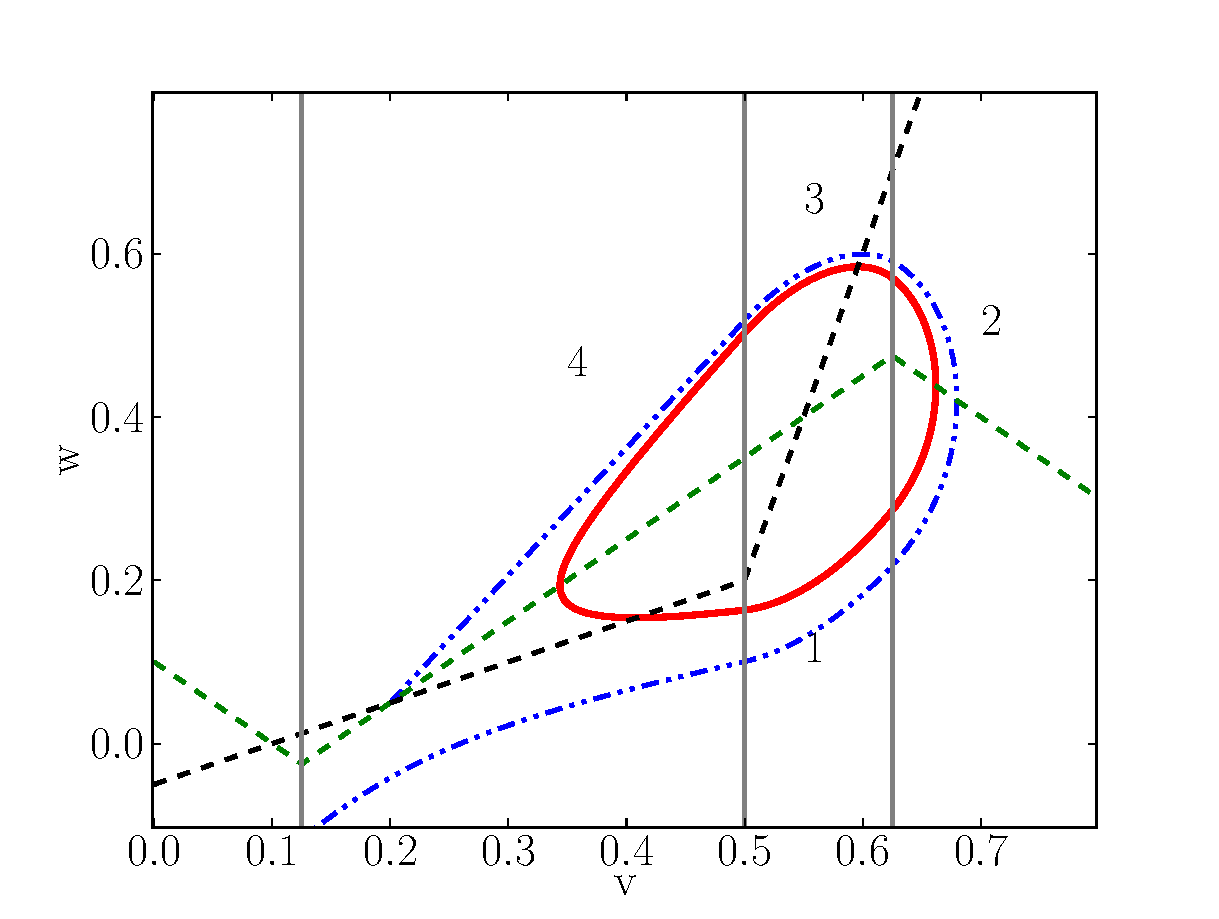
\includegraphics[width=.8\textwidth]{pml_fig.pdf}
 \caption{Piecewise Morris-Lecar model (Coombes 2008).}
\end{figure}
\end{frame}



\begin{frame}


Following the notation in Coombes and by Theorem 1, we can calculate discontinuities over the boundary by the relation
\begin{equation}
 Q_\mu(T_\mu)M^{R=\mu}= \ Q_\mu(0).
\end{equation}
We will calculate the matrix $M^R$ for each boundary starting with the boundary between regions 4 and 1.  To avoid possible confusion with the matrix exponent, we define $M_R := M^R$.



\end{frame}

\begin{frame}
Consider the boundary between regions $4$ and $1$,
\begin{equation}
 Q_1(0) = M_4 Q_4(T_4).
\end{equation}

\begin{equation}
\begin{split}
 M_4 &= \matrix{cc}{f_0^1 & A_4\\0 & 1}^{-1} \matrix{cc}{f_f^4 & A_4\\0 & 1}\\
 &=\matrix{cc}{f_f^4/f_0^1 & 0\\0 & 1}.
\end{split}
\end{equation}

By definition,
\begin{equation}
\begin{split}
 f_f^4/f_0^1 &= \frac{-v_{th}^1 - w^* + I}{v_{th}^1-a-w^*+I}\\
 &= \frac{-a/2 - w^* + I}{a/2-a-w^*+I} = 1,
\end{split}
\end{equation}

\end{frame}

\begin{frame}
 \begin{figure}
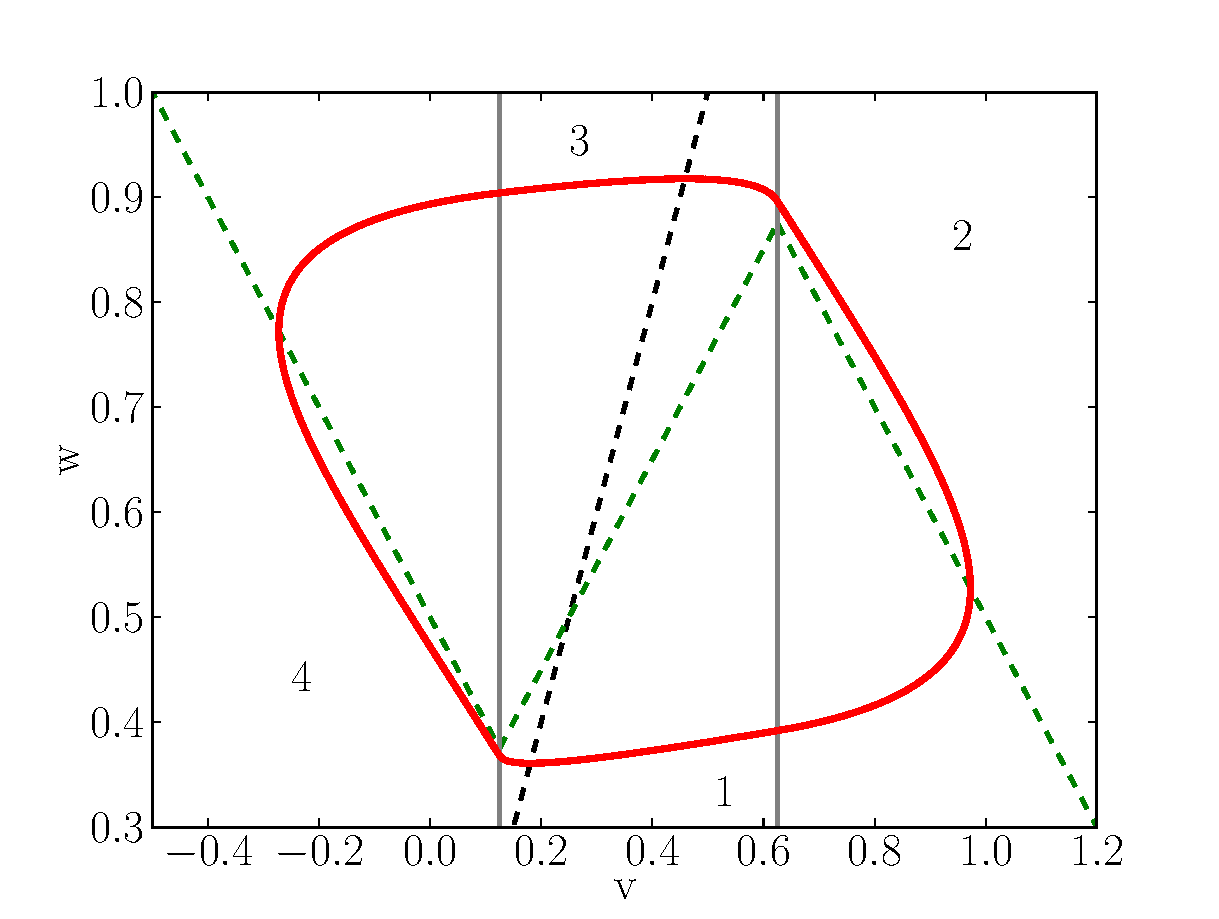
\includegraphics[width=\textwidth]{pmk_fig.pdf}
\caption{McKean Model (Coombes 2008)}\end{figure}
\end{frame}



\begin{frame}
\frametitle{\insertsection}
\framesubtitle{\insertsubsection}
Iris system.  Suppose the lower left square of the iris system is region $R=1$.  We can use the normalization condition 
\begin{equation}\label{eq:normalization}
F_0^R\cdot z^R_0=\frac{1}{T},
\end{equation}

with the result above to derive a unique expression for the iPRC of the iris system.  In order for the normalization condition to hold, we must have
\begin{align}
 z_1(0) &= \frac{c}{\lambda},\\
 z_2(0) &= \frac{c+1/T}{u}.
\end{align}
\end{frame}

\begin{frame}
From our theorem, at the boundary between regions 1 and 2 (between the Southwest and Northwest squares), $\psi = \pi/2$, so
\begin{equation}
 M^R = \matrix{cc}{1 & 0\\ \frac{f_f^R-f_0^{R+1}}{g_0^{R+1}} & \frac{g_f^R}{g_0^{R+1}}}.
\end{equation}

In particular, this matrix gives me the relationship $z_1^{R+1}(0) = z_1^R(t_{final})$.  Horizontal perturbations in the Northwest square are equivalent to vertical perturbations in the Southwest square, so we must have that (in terms of phase)
\begin{equation}
 z_1(1) = z_2(0).
\end{equation}
\end{frame}

\begin{frame}

Since we have (for region R)
\begin{equation}
 \frac{dz}{dt} = -(DF(t))^T z(t) = \matrix{cc}{\lambda & 0\\ 0 & -1} z(t),
\end{equation}
the solutions are (in terms of phase)
\begin{equation}
\begin{split}
 z_1(\theta) &= z_1(0) u^{-\lambda \theta},\\
 z_2(\theta) &= z_2(0) u^{\theta}.\\
\end{split}
\end{equation}
Since
\begin{equation}
\begin{split}
 z_1(1) = z_1(0) u^{-\lambda},
\end{split}
\end{equation}
we need to solve
\begin{equation}
\begin{split}
  z_1(0)u^{-\lambda} &= z_2(0)\\
  \frac{c}{\lambda} u^{-\lambda} &= \frac{c+1/T}{u}.
\end{split}
\end{equation}


\end{frame}

\begin{frame}
When we solve for the constant $c$, we get
\begin{equation}
 c  = \frac{1}{T}\left (\frac{\lambda u^\lambda}{u - \lambda u^\lambda}\right ).
\end{equation}

Plugging this constant into the formula for the iPRC, we (re-)derive both components of the iPRC for the iris system.  For the first component we have
\begin{equation}
\begin{split}
 z_1(\theta) &= z_1(0)e^{\lambda \theta T} = \frac{c}{\lambda}e^{\lambda \theta T} \\
 &=\frac{1}{T}  \left (\frac{u^\lambda}{u- \lambda u^\lambda}\right ) u^{-\lambda \theta}\\
 &=\frac{u^{\lambda(1-\theta)}}{T(u- \lambda u^\lambda)}.
\end{split}
\end{equation}
\end{frame}

\begin{frame}
Using the same value of $c$, 
\begin{equation}
  Z_2(0) = \frac{1}{T (u-\lambda u^\lambda)},
\end{equation}
so
\begin{equation}
 Z_2(\theta) =\frac{u^{\theta}}{T (u-\lambda u^\lambda)}.
\end{equation}
\end{frame}

\begin{frame}
\frametitle{\insertsection}
Future work
\begin{itemize}
 \item Use this theorem to predict a (numerical) value for the jump in the iPRC for the iris system
 \item Apply this theorem to other piecewise linear systems (McKean, Piecewise Morris-Lecar,Glass networks)
\end{itemize}
\end{frame}



% \subsection{Summary of Shaw et al. (2012)}

% \subsubsection{Models}
%   \begin{frame}
% 	 \frametitle{\insertsection}
%     	\framesubtitle{\insertsubsection}
%     	We primarily use three planar models for much of our numerical and analytical analyses: The sine, iris, and Morris-Lecar systems.
%     	The sine system is defined as
% \begin{equation}\begin{split}\frac{dy_1}{dt} &= f(y_1,y_2) + \mu g(y_1,y_2),\\ \frac{dy_2}{dt} &= g(y_1,y_2) - \mu f(y_1,y_2), \end{split}\end{equation}
% 
%   where \begin{equation}
%          \begin{split}
%           f(y_1,y_2) &= \cos(y_1)\sin(y_2)+ \alpha \sin(2y_1),\\
%           g(y_1,y_2) &= -\sin(y_1)\cos(y_2)+\alpha \sin(2y_2),
%          \end{split}
%         \end{equation}
%         
%         and $\mu$ acts as the bifurcation parameter.  The system exhibits a heteroclinic bifurcation (cycle) when $\mu = 0$ and a stable limit cycle for $0< \mu \ll 1$.
%   \end{frame}
%   
%   \begin{frame}
%  \frametitle{\insertsection}
%     	\framesubtitle{\insertsubsection}
%     	In Shaw et al. (2012), we derive several analytical results for the iris system.  The iris system is a piecewise linear planar dynamical system.  It can be defined by a local vector field
% \begin{equation}\begin{split} \frac{ds}{dt} &= -\lambda s,\\ \frac{du}{dt} &= u. \end{split}\end{equation}
% 
%   Solutions are exponential functions, allowing for analytical solutions to some problems.
%   
%   \end{frame}
%     \begin{frame}
%  \frametitle{\insertsection}
%     	\framesubtitle{\insertsubsection}
%     	Generate limit cycles by rotating the vector field with an offset value $a$.
%     	\begin{figure}
%     	 \includegraphics[width=.5\textwidth]{iris_b_fig.pdf}
%     	 \includegraphics[width=.5\textwidth]{iris_c_fig.pdf}
%     	\caption{Left: $a=0.05$.  Right: $a=0.2$.}\end{figure}
% 
%   \end{frame}
%   
% \begin{frame}
%  \frametitle{\insertsection}
%  \framesubtitle{\insertsubsection}
% We derived an analytical expression for the iPRC of the iris system.
% 
% \begin{figure}
%  \includegraphics[width=.6\textwidth]{iris_prc_fig.pdf}
%   %\includegraphics[width=.5\textwidth]{morris-lecar_prcs-revised.pdf}
% \end{figure}
% \end{frame}

%   \begin{frame}
% 	 \frametitle{\insertsection}
%     	\framesubtitle{\insertsubsection}
% 	\begin{itemize}
% 	\item Analytic expression for the iPRC of the iris system
% 	\item Qualitative resemblance in numerical iPRC of Morris-Lecar system
% 	\end{itemize}
%   \end{frame}

%\subsubsection{iPRC in terms of arc length}
% \begin{frame}
%  \frametitle{\insertsection}
%  \framesubtitle{\insertsubsection}
% \begin{figure}
%  \includegraphics[width=.8\textwidth]{../iprc_al.pdf}
%  % \includegraphics[width=.5\textwidth]{morris-lecar_prcs-revised.pdf}
% \caption{The iPRC diverges and the kink (arc length 3) becomes more pronounced closer to the bifurcation.}\end{figure}
% \end{frame}

% \section{A rapid change in the iPRC in terms of arc length: Proof of convergence}
% 
% \begin{frame}
% \frametitle{Table of Contents}
% \tableofcontents[currentsection]
% \end{frame}
% 
% 
%   \begin{frame}
%  \frametitle{\insertsection}
%     \framesubtitle{\insertsubsection}
%     
% \begin{definition}
%  The arc length function $L$ of the iris system is defined by the integral
%  
%  \begin{equation}
%   L(\phi) = \int_0^{\phi T} \! \sqrt{(-\lambda s_0 e^{-\lambda s})^2 + (u_0 e^s)^2} \, \mathrm{d}s
%  \end{equation}
% 
% \end{definition}
% 
% \begin{Lemma}
%  The arc length function of the iris system converges to the step function in the limit of the heteroclinic bifurcation.
% \end{Lemma}
% 
% \begin{Lemma}
% The iPRC of the iris system diverges for perturbations along arc length $L < 1$ and converges to zero for perturbations along arc length $L > 1$.
% \end{Lemma}
%   \end{frame}
%   
%   \subsection{Proof in the special case of the iris system}
%   
% \begin{frame}
% \frametitle{\insertsection}
% \framesubtitle{\insertsubsection}
% \textit{Proof of first lemma}. The walls of the iris system are of unit length, we just need to show that all phases $\phi \in (0,1)$ converge to unit arc length in the limit of the heteroclinic bifurcation.  We can do this by showing
% 
% \begin{equation}
%   \forall \varepsilon > 0, \exists u >0\,\, \text{s.t.} ||(x,y)||_1 < 2\varepsilon,  
% \end{equation}
% where $(x,y)$ is a point corresponding to an arbitrary phase $\hat\phi \in (0,1)$ of a limit cycle with entry coordinate $(1,u)$. Given $(1,u)$, we know there exists a bifurcation parameter $a$ for which $(1,u)$ lies on a limit cycle.
%   \end{frame}
%   
%   
% \begin{frame}
% \frametitle{\insertsection}
% \framesubtitle{\insertsubsection}
% 
% Given an arbitrary coordinate $(x,y)$ (with corresponding $\hat\phi$), we can find the entry coordinate $u$ by the relation
% 
% \begin{equation}
%  u = y x^{1/\lambda}.
% \end{equation}
% 
% Moreover, we can find a direct relationship between the arbitrary coordinates $(x,y)$.
% \begin{equation}
% y  =x^{\frac{1}{\lambda}(\frac{1}{\hat\phi} - 1)}.
% \end{equation}
% 
% Combining these equations yield equations for $x$ and $y$ in terms of the entry coordinate $u$.
% \begin{equation}
% \begin{split}
% x &= u^{\lambda \hat\phi},\\
% y &= u^{(1-\hat{\phi})}.
% \end{split}\label{eqs:x-u-y-u}
% \end{equation}
% \end{frame}
% 
% 
% 
% 
% \begin{frame}
% \frametitle{\insertsection}
% \framesubtitle{\insertsubsection}
% % \leq \varepsilon^4 < \varepsilon$.
% In order to show convergence, let $0 < \varepsilon \ll 1$ be given.  Define $u = \varepsilon^{1/(\hat{\phi}(1-\hat{\phi}))}$.  By Eq.~\eqref{eqs:x-u-y-u}, we have
% \begin{equation}
% \begin{split}
%   |x| + |y| &= |u^{\lambda \hat{\phi}}| + |u^{1-\hat{\phi}}| \\
%   &= \varepsilon^{\lambda/(1-\hat{\phi})} + \varepsilon^{1/\hat{\phi}} \\
%   &< \varepsilon + \varepsilon = 2\varepsilon.
% \end{split}
% \end{equation}
% 
% This holds for each $\varepsilon >0$, so $||(x,y)||_1 \rightarrow 0$ as $\varepsilon \rightarrow 0$. $\Box$
% \end{frame}
% 
%   \begin{frame}
%    \frametitle{\insertsection}
% \framesubtitle{\insertsubsection}
% \textit{Proof of second lemma}.  In order to find an analytical solution to the iPRC in terms of arc length, we need to invert the arc length function.  Since the arc length function converges (pointwise) to a step function, I can use the following piecewise approximation
% 
% \begin{figure}
%  \includegraphics[width=.7\textwidth]{pwla.png}
%  \caption{Blue: arc length function.  Red: Piecewise linear approximation}\end{figure}
% 
%   \end{frame}
%   
%     \begin{frame}
%    \frametitle{\insertsection}
% \framesubtitle{\insertsubsection}
% 
% Now that we have an expression to transform arc length into phase ($L_i^{-1} : L \mapsto \phi$), we can plug in the transformation into the iPRC.  This yields the following equations, which diverge or converge according to the comparison test.
% 
% (note that $\log(1/u)u^a \rightarrow 0$ as $u \rightarrow 0$ for any $a > 0$)
% 
% \begin{equation}
% \begin{split}
%\phi \leq \overline{\phi}_{1,2}
%\phi \geq \overline{\phi}_{2,3}
%   Z_{y,1}(L_1^{-1}(L)) &\geq \frac{1}{\log(1/u) u^{1/2} (1-\lambda u^{\lambda-1})} \rightarrow \infty,\\
%  Z_{y,3}(L_3^{-1}(L)) &\leq \frac{1}{\log(1/u) (1-\lambda u^{\lambda-1})} \rightarrow 0.
% \end{split}
% \end{equation}
% \end{frame}
% 
% \subsection{Possible generalizations and applications}
%   \begin{frame}
%  \frametitle{\insertsection}
%     	\framesubtitle{\insertsubsection}
% We might be able to apply this result to general homoclinic systems if
% \begin{itemize}
%  \item We can transform the general system to resemble an iris square
%  \item We can predict the effects of perturbations outside a small neighborhood of the saddle
%  \item We know how perturbations in the transformed space relate to perturbations in the untransformed space
% \end{itemize}
% 
%   \end{frame}

\begin{frame}
        \frametitle{References}
        \bibliographystyle{plain}
        \bibliography{math,PJT}
\end{frame}



\begin{frame}
\frametitle{Acknowledgements}
Thanks to Dr. Peter J. Thomas, Dr. Hillel J. Chiel, Kendrick Shaw, and my other committee members, Dr. Alethea Barbaro and Dr. Michael Hurley.
\end{frame}

\end{document}